\section{Experiments}
\label{experiments}

\subsection{Experimental Setup}
\label{experimentalsetup}
There two steps during training process.
The first step is to train difference kinds of RCNN to get the best combination between CNN models and LSTM, the outputs from RCNN($1 \times 256$) will be feed into two fully connected layers to get classification results, as shown in Fig~\ref{onestream}. We compare three kinds of classic CNN models: VGG16, GoogLeNet with Inception-V3, ResNet50. Experiments show that ResNet50 has the best performance. We tried to use deeper network like ResNet101, however using ResNet101 makes the training of model very slow and bring a heavy burden to servers. So we decide to use ResNet50 in RCNN. Moreover, we use CNN models pre-trained on ImageNet \cite{ILSVRC15}. Models without pre-training is almost impossible to train because it won't converge or converge very slow during training. We test difference RCNNs, and experiments show that using pre-trained models can significantly improve the converging speed, as shown in Table~\ref{pretrain}.

The second step is to train MDDNet model. We use RCNN get in the first step as encoder for CT scan visual features, use LSTM as feature encoder for complaints, and combine them with information of age and gender. All these features will be feed into two fully-connected layers and one Softmax layer to get final classification results. Initial learning rate is set to 0.0005 and drops 50\% every 3000 training steps. The dropout rate in fully-connected layers is set to 0.5.

MDDNet will be trained for 4 epoch, and each epoch contains 15 iteration for all training data.

\begin{table}[htb]
\vspace{-0cm}
\caption{Comparison between Training from Scratch and Training with Pre-trained Weights}
\vspace{-0cm}
\begin{center}
    \begin{tabular}{|c|c|c|c|}
    \hline
    \textbf{\textit{Structure}} & \textbf{\textit{Pre-trained}} & \textbf{\textit{Data}}& \textbf{\textit{Accuracy}}  \\
    \hline
    RCNN(ResNet) &No & Lung Window Image & 0.545\\
    RCNN(GoogLeNet) & No & Lung Window Image & 0.545\\
    RCNN(ResNet) & Yes & Lung Window Image & 0.925\\
    RCNN(GoogLeNet) & Yes & Lung Window Image & 0.865\\
    
    \hline
    \end{tabular}
\vspace{-0cm}
\label{pretrain}
\end{center}
\vspace{-0cm}
\end{table}



\subsection{Effectiveness of Three-Channel Image}
\label{effectiveness}
In order to verify the effectiveness of three-channel pre-processing, we train four RCNNs with three-channel images, lung window images, high attenuation images and low attenuation images and output the feature maps of convolutional layer. Sample feature mapes are shown in Fig~\ref{show}. More specificity, we output the feature maps after one convolutional layer, one max pooling layer, and three ResNet blocks, the size of feature maps are $128 \times 128$. In order to keep experiments environment consistent, all experiments carried on in this part are based on RCNN with ResNet50. We can see that CNN trained by three-channel images has advantages over CNNs trained by other kinds of images as shown in Fig~\ref{show}. 

In Fig~\ref{show}, images in the first column are original fake color CT images, which are direct outputs from CT slices. The second, the third and the forth columes are feature maps from lung window CNN, high attenuation CNN and low attenuation CNN. Images in the last colume are feature mapes from three-channel CNN.

\begin{figure*}[t]
    \centerline{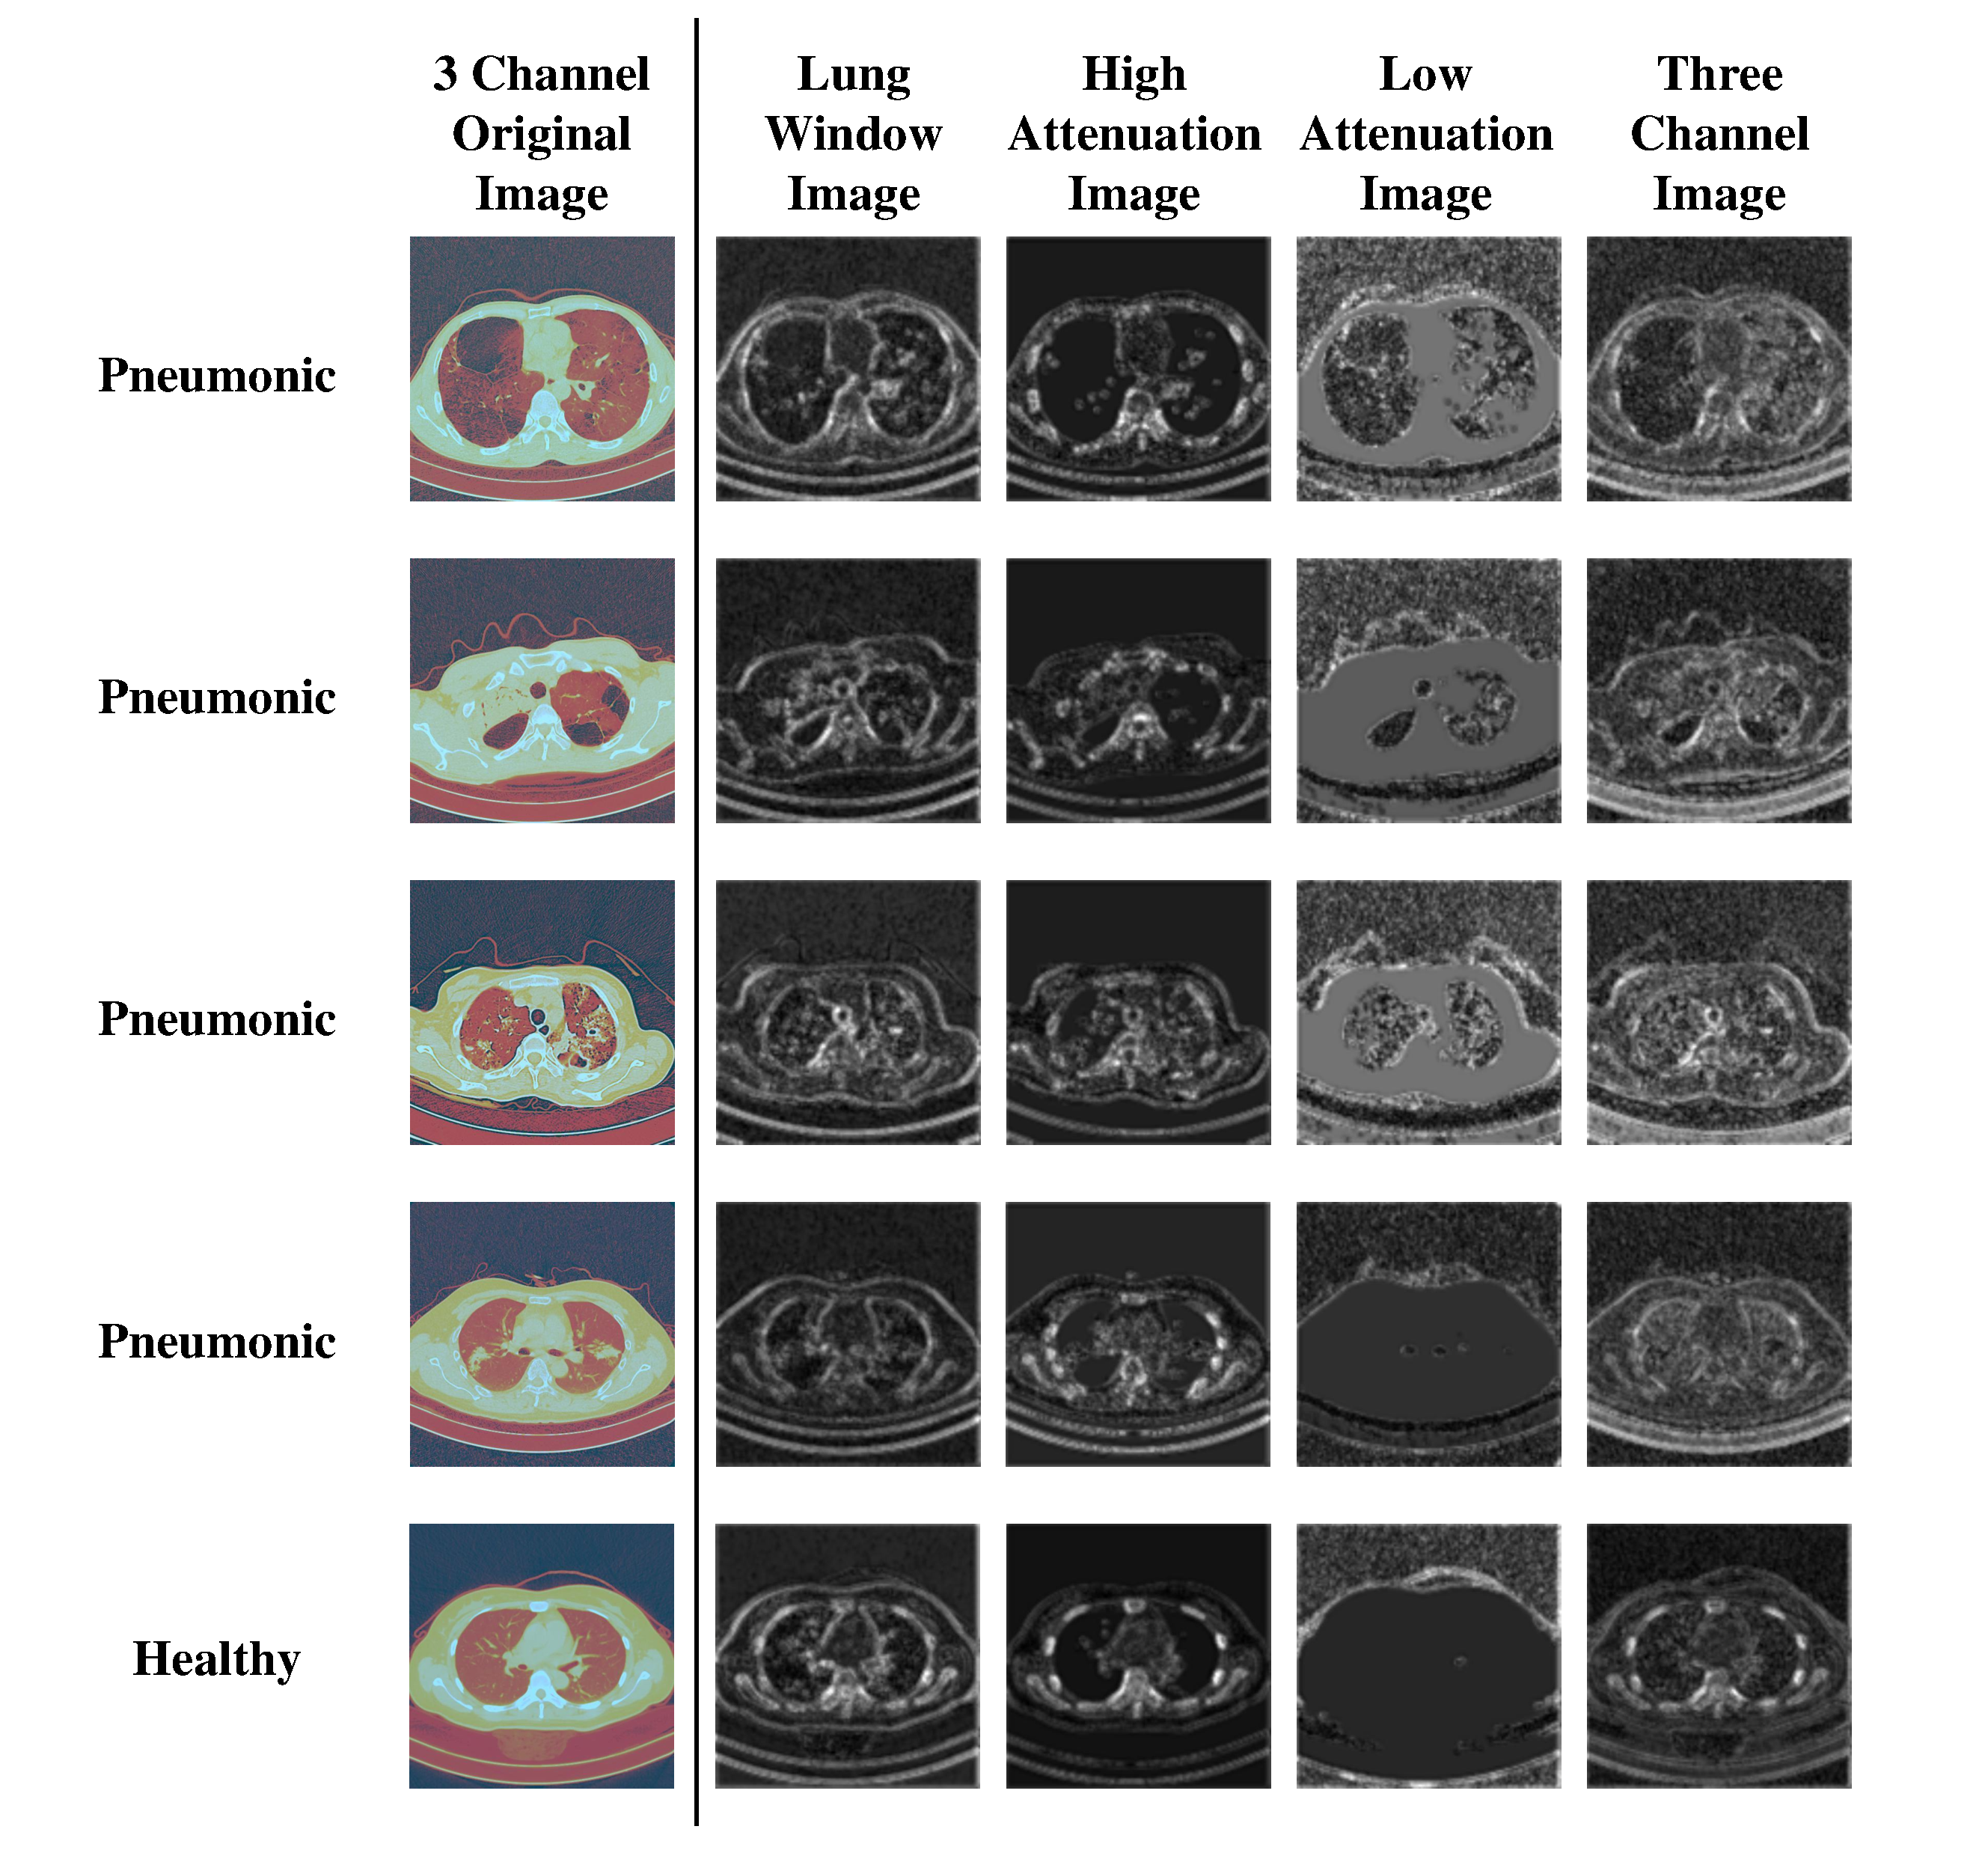
\includegraphics[width=180mm]{show.pdf}}
    \vspace{-0cm}
    \caption{Convolutional Feature Maps from CNN Models Trained by Different Images. In the first and the second rows, three-channel CNN can capture the low dense tissues of lungs, which are not very clear in lung window CNN and high attenuation CNN. Low attenuation CNN can notice the low dense tissues, but apparently the details of heart and vessels are ignored in the loa attenuation CNN. 
    In the third and the forth row, three-channel CNN still has ability to capture high dense tissues, which is the same as normal CNN and high attenuation CNN, but low attenuation CNN has difficulty in doing so. In the third row, low attenuation CNN cannot distinguish the normal and unnormal tissues. Moreover, in the forth row, low attenuation CNN ignores high dense tissues. The last row shows a healthy case. Healthy case has a clear view in lung window CNN, high attenuation CNN and three-channel CNN, but shows nothing in low attenuation CNN.}
    \vspace{-0cm}
    \label{show}
    \end{figure*}

\subsection{Effectiveness of Complaints, Age and Gender}
\label{complaintsagegender}
As mentioned in \ref{intro}, information about age, gender and complaints can enhance the features extracted from CT image or become a supplement. Complaints can provied information like symptoms, location.
We count word frequency about symptoms. The frequency is shown in Table~\ref{frequency1} and Table~\ref{frequency2}. We can see that top 10 key words in healthy cases and pneumonic cases have certain regularity. `Cough' is the most frequent key word in both HC(healthy cases) and PC(pneumonic cases). It apperas 256 times(46.4\%) in PC, 183 times(40.7\%) in HC. However, symptoms like `Expectoration', `Fever', `Coughing blood' appear more frequently in PC. For example, `Coughing blood' appears 47 times in PC, but only appears 1 time in HC.


\begin{table*}[htb]
    \vspace{-0cm}
    \caption{Top 10 Frequent Key Words in Pneumonia Cases}
    \vspace{-0cm}
    \begin{center}
    \begin{tabular}{|c|c|c|c|c|}
        \hline
        \textbf{\textit{Key Words}} & \textbf{\textit{Frequency in PC}} & \textbf{\textit{Percentage}}& \textbf{\textit{Frequency in HC}}& \textbf{\textit{Percentage}} \\
    \hline
    \begin{CJK}{UTF8}{gbsn}\textbf{咳嗽}\end{CJK}, \textbf{Cough} & 256 & 0.464 & 183 & 0.407\\
    \begin{CJK}{UTF8}{gbsn}\textbf{咳痰}\end{CJK}, \textbf{Expectoration} & 103 & 0.187 & 42 & 0.093\\
    \begin{CJK}{UTF8}{gbsn}\textbf{反复}\end{CJK}, \textbf{Repeat Condition} & 65 & 0.118 & 48 & 0.107\\
    \begin{CJK}{UTF8}{gbsn}\textbf{气促}\end{CJK}, \textbf{Shortness of Breath} & 60 & 0.109 & 17 & 0.038\\
    \begin{CJK}{UTF8}{gbsn}发热\end{CJK}, Fever & 51 & 0.092 & 14 & 0.031\\
    \begin{CJK}{UTF8}{gbsn}咯血\end{CJK}, Coughing Blood & 47 & 0.085 & 1 & 0.002\\
    \begin{CJK}{UTF8}{gbsn}加重\end{CJK}, Aggravation & 46 & 0.081 & 13 & 0.029\\
    \begin{CJK}{UTF8}{gbsn}\textbf{痰}\end{CJK}, \textbf{Sputum} & 32 & 0.058 & 19 & 0.042\\
    \begin{CJK}{UTF8}{gbsn}乏力\end{CJK}, Weak& 29 & 0.053 & 7 & 0.016\\
    \begin{CJK}{UTF8}{gbsn}感染\end{CJK}, Infection& 28 & 0.051 & 1 & 0.002\\
    
    \hline
    \end{tabular}
    \vspace{0.1cm}
    \label{frequency1}\\
    \footnotesize{Percentage is frequency divided by number of cases. PC is Pneumonic Cases. HC is Healthy Cases}

    \end{center}
    \vspace{-0.0cm}
    \end{table*}

    \begin{table*}[htb]
        \vspace{-0cm}
        \caption{Top 10 Frequent Key Words in Healthy Cases}
        \vspace{-0cm}
        \begin{center}
        \begin{tabular}{|c|c|c|c|c|}
            \hline
            \textbf{\textit{Key Words}} & \textbf{\textit{Frequency in HC}} & \textbf{\textit{Percentage}}& \textbf{\textit{Frequency in PC}}& \textbf{\textit{Percentage}} \\
        \hline
        \begin{CJK}{UTF8}{gbsn}\textbf{咳嗽}\end{CJK}, \textbf{Cough},  & 183 & 0.407 & 256 & 0.464\\
        \begin{CJK}{UTF8}{gbsn}胸痛\end{CJK}, Chest Pain & 67 & 0.149 & 17 & 0.031\\
        \begin{CJK}{UTF8}{gbsn}不适\end{CJK}, Unconfortable & 54 & 0.120 & 25 & 0.045\\
        \begin{CJK}{UTF8}{gbsn}疼痛\end{CJK}, Pain & 53 & 0.118 & 25 & 0.045\\
        \begin{CJK}{UTF8}{gbsn}\textbf{反复}\end{CJK}, \textbf{Repeat Condition} & 48 & 0.107 & 65 & 0.118\\
        \begin{CJK}{UTF8}{gbsn}\textbf{咳痰}\end{CJK}, \textbf{Expectoration} & 42 & 0.093 & 103 & 0.187\\
        \begin{CJK}{UTF8}{gbsn}背痛\end{CJK}, Backache & 28 & 0.062 & 8 & 0.014\\
        \begin{CJK}{UTF8}{gbsn}\textbf{痰}\end{CJK}, \textbf{Sputum}& 19 & 0.042 & 32 & 0.058\\
        \begin{CJK}{UTF8}{gbsn}胸闷\end{CJK}, Chest Tightness & 19 & 0.042 & 16 & 0.029\\
        \begin{CJK}{UTF8}{gbsn}\textbf{气促}\end{CJK}, \textbf{Shortness of Breath}& 17 & 0.038 & 60 & 0.109\\
        
        \hline
        \end{tabular}
        \vspace{0.1cm}
        \label{frequency2}\\
        \footnotesize{Percentage is frequency divided by number of cases. PC is Pneumonic Cases. HC is Healthy Cases}
    
        \end{center}
        \vspace{-0.0cm}
        \end{table*}

Information provided by complaints is also related to CT images. In Fig~\ref{txtpic}, we can see that according to the location and symptom information provided by complaints, we can accurately locate lesions in CT. It means information from complaints is related to CT images and can assist deep learning model.

\begin{figure*}[t]
    \centerline{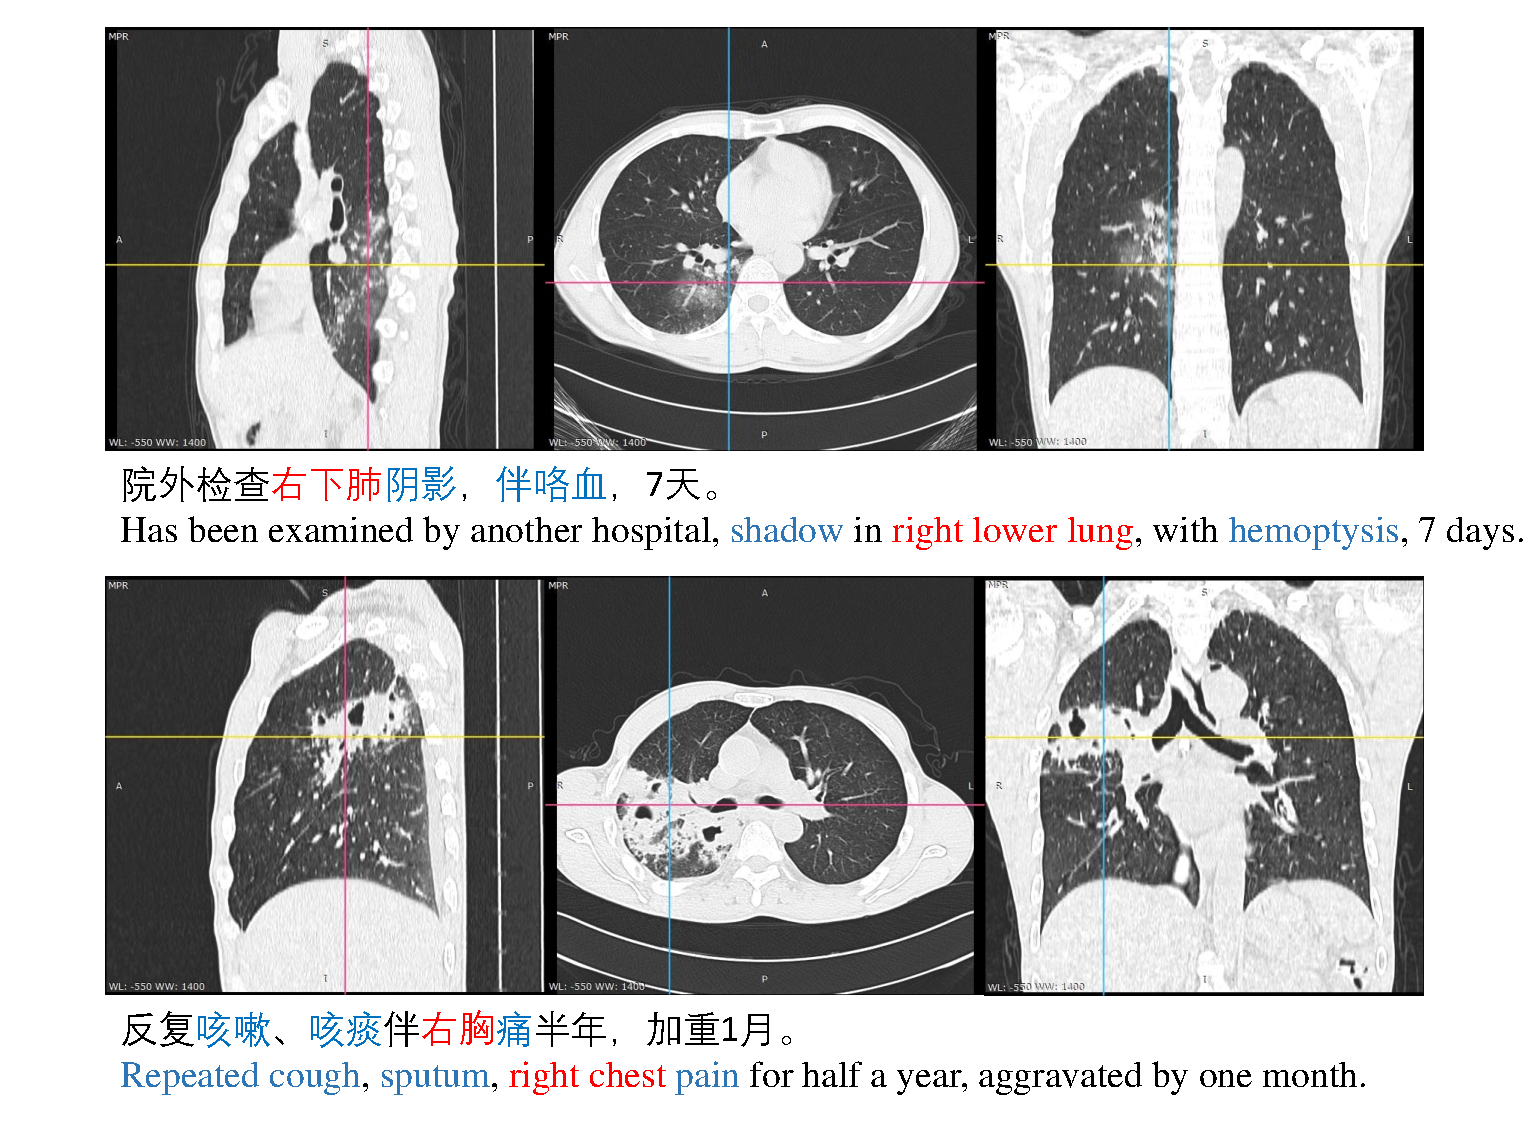
\includegraphics[width=180mm]{txtpic.pdf}}
    \vspace{-0cm}
    \caption{Complaints can provide information that related to CT images. In this figure, we show two cases which are pneumonic, each case has complaints provided by patients. Words marked red provide location, words marked blue provide symptoms. English complaints are translated from Chinese complaints above. We can see that location and symptoms information provided by complaints are related to abnormal tissues in CT images.}
    \vspace{-0cm}
    \label{txtpic}
    \end{figure*}

\subsection{Results}
\label{results}
In order to prove the effect of three-channel images, auxiliary loss and Multimodal Data, we run a lot of experiments to compare with each other, and the results of experiments is shown in Table~\ref{comparison}.

First of all, we run experiments to prove the effect of images with three ranges of HU values and choose the best architecture of RCNN. We can see that RCNN(ResNet), RCNN(GoogLeNet) and RCNN(VGG) trained by three-channel image all have better performance than these models trained by one-channel data. 
For RCNN(VGG), model trained by three-channel image outperforms RCNN(VGG) trained by lung window image in accuracy, specificity and AUROC score. RCNN(VGG) trained by lung window image has better performance in sensitivity, but we can see that it only get 0.626 in specificity, which means this model has not been trained well. 

For RCNN(ResNet) and RCNN(GoogLeNet), we can see that these two models trained by three-channel image perform best compared to those trained by lung window image, high attenuation image and low attenuation image. Especially RCNN(ResNet) trained by three-channel image, it get 0.930 in accuracy, 0.934 in specificity, which are highest in different RCNN. RCNN(ResNet) trained by lung window image has 0.954 in sensitivity, which is the highest in experiments, but it only achieves 0.890 in specificity and corrupts the performance of whole model. As a result, we use RCNN(ResNet) as our visual feature encoder for CT.

Then we run a experiment to prove the effectiveness of auxiliary loss. We train RCNN(ResNet) with three channel image, but we set $\omega$ to $1$, which means we remove the gradient propagates directly to CNN, this model actually has only one loss. We can see that the performance of RCNN with single loss drops around 1\% in all four indications. It proves that, by using auxiliary loss, CNN will be trained in a better way. 

At last, we run experiments to prove that Multimodal Data can enhance the performance of CAD system. As shown in section~\ref{MMDD}, the output of RCNN($1 \times 256$), features of complaints($1 \times 50$), gender($1 \times 1$) and age($1 \times 1$) will be concatenated together($1 \times 308$) and fused by two fully-connected layers. It is simple, but effective. We can see that MDDNet has the highest score in accuracy, specificity and AUROC score. But it achieves 0.936 in sensitivity, 1.8\% lower than the highest 0.954. It means MDDNet has the best performance of binary classification according to its AUROC score. We also remove the information about age and gender, we found that MDDNet without age and gender has a higher sensitivity and lower specificity than MDDNet with information about age and gender. 
\begin{table*}[htb]
    \vspace{-0cm}
    \caption{Comparison of All Kinds of RCNN and MDDNet}
    \vspace{-0cm}
    \begin{center}
    \begin{tabular}{|c|c|c|c|c|c|c|}
    \hline
    \textbf{\textit{Structure}} & \textbf{\textit{Data}}& \textbf{\textit{Accuracy}}  & \textbf{\textit{Sensitivity}} & \textbf{\textit{Specificity}} & \textbf{\textit{AUROC}}& \textbf{\textit{AUROC Rank}}\\
    \hline
    RCNN(VGG) & Lung Window Image & 0.805 & {\bfseries 0.954} &0.626 &0.790 &13\\
    RCNN(GoogLeNet) & Lung Window Image& 0.865 & 0.826 & 0.912 & 0.869 &10\\
    RCNN(ResNet) & Lung Window Image & 0.925 & {\bfseries 0.954} & 0.890 & 0.922 &4\\
    RCNN(GoogLeNet) & High Attenuation Image& 0.880 & 0.853 & 0.912 & 0.883 &8\\
    RCNN(ResNet)& High Attenuation Image& 0.875 & 0.908 & 0.835 & 0.872 &9\\
    RCNN(GoogLeNet) & Low Attenuation Image& 0.860 & 0.890 & 0.824 & 0.857 &12\\
    RCNN(ResNet) & Low Attenuation Image& 0.865 & 0.900 & 0.824 & 0.861 &11\\
    RCNN(VGG) & Three Channel Image& 0.890 & 0.927 &0.846 &0.886 &7\\
    RCNN(GoogLeNet)& Three Channel Image & 0.905 & 0.900 & 0.912 & 0.906 &6\\
    RCNN(ResNet) & Three Channel Image& 0.930 & 0.927 & 0.934 & 0.930 &2\\
    RCNN(ResNet), One Loss & Three Channel Image& 0.920 & 0.917 & 0.923 & 0.920 &5\\
    MDDNet & Three Channel Image \& Complaints & 0.925 & 0.945 & 0.901 & 0.923 &3\\
    MDDNet & Multimodal Data&  {\bfseries 0.945} & 0.936 & {\bfseries 0.956} & {\bfseries 0.945} &1\\
    \hline
    \end{tabular}
    \vspace{-0cm}
    \label{comparison}
    \end{center}
    \vspace{-0cm}
    \end{table*}
